\RequirePackage[l2tabu, orthodox]{nag}
\RequirePackage{silence}
\WarningFilter{fmtcount}{\ordinal already defined use \FCordinal instead}
\documentclass[english, french]{beamer}
%INSTALL

%avoids a warning
\usepackage[log-declarations=false]{xparse}
\usepackage{fontspec} %font selecting commands
\usepackage{xunicode}
%warn about missing characters
\tracinglostchars=2

%REDAC
\usepackage{booktabs}
\usepackage{calc}

\usepackage{mathtools} %load this before babel!
	\mathtoolsset{showonlyrefs,showmanualtags}

\usepackage{babel}
%suppresses the warning about frenchb not modifying the captions (“—” to “:” in “Figure 1 – Legend”).
	\frenchbsetup{AutoSpacePunctuation=false,SuppressWarning=false}

\usepackage[super]{nth}
\usepackage{listings} %typeset source code listings
	\lstset{language=XML,tabsize=2,literate={"}{{\tt"}}1,captionpos=b}
\usepackage[nolist,smaller,printonlyused]{acronym}%,smaller option produces warnings from relsize in some cases, it seems.
\usepackage[nodayofweek]{datetime}%must be loaded after the babel package
\usepackage{xspace}
\usepackage{hyperref}% option pdfusetitle must be introduced here, not in hypersetup.
%breaklinks makes links on multiple lines into different PDF links to the same target.
%colorlinks (false): Colors the text of links and anchors. The colors chosen depend on the the type of link. In spite of colored boxes, the colored text remains when printing.
%linkcolor=black: this leaves other links in colors, e.g. refs in green, don't print well.
%pdfborder (0 0 1, set to 0 0 0 if colorlinks): width of PDF link border
%hidelinks
\hypersetup{breaklinks,bookmarksopen,colorlinks=true,urlcolor=blue,linkcolor=,hyperfigures=true}
% hyperref doc says: Package bookmark replaces hyperref’s bookmark organization by a new algorithm (...) Therefore I recommend using this package.
\usepackage{bookmark}

% center floats by default, but do not use with float
% \usepackage{floatrow}
% \makeatletter
% \g@addto@macro\@floatboxreset\centering
% \makeatother
\usepackage{ragged2e} %new com­mands \Cen­ter­ing, \RaggedLeft, and \RaggedRight and new en­vi­ron­ments Cen­ter, FlushLeft, and FlushRight, which set ragged text and are eas­ily con­fig­urable to al­low hy­phen­ation (the cor­re­spond­ing com­mands in LaTeX, all of whose names are lower-case, pre­vent hy­phen­ation al­to­gether). 
\usepackage{siunitx} %[expproduct=tighttimes, decimalsymbol=comma]
\sisetup{detect-all}% to detect e.g. when in math mode (use a math font)
\usepackage{braket} %for \Set
\usepackage{natbib}

\usepackage{amsmath,amsthm}
% \usepackage{amsfonts} %not required?
% \usepackage{dsfont} %for what?
%unicode-math overwrites the following commands from the mathtools package: \dblcolon, \coloneqq, \Coloneqq, \eqqcolon. Using the other colon-like commands from mathtools will lead to inconsistencies. Plus, Using \overbracket and \underbracke from mathtools package. Use \Uoverbracket and \Uunderbracke for original unicode-math definition.
%use exclusively \mathbf and choose math bold style below.
\usepackage[warnings-off={mathtools-colon, mathtools-overbracket}, bold-style=ISO]{unicode-math}

\defaultfontfeatures{
	Fractions=On,
	Mapping=tex-text% to turn "--" into dashes, useful for bibtex%%
}
\defaultfontfeatures[\rmfamily, \sffamily]{
	Fractions=On,
	Mapping=% to leave " alone (disable the default mapping tex-text; requires loading the font afterwards?)
}
\newfontfamily\xitsfamily{XITS}
\newfontfamily\texgyretermesfamily{TeX Gyre Termes}
\newfontfamily\texgyreherosfamily{TeX Gyre Heros}
\newfontfamily\lmfamily{Latin Modern Roman}
\setmainfont{Latin Modern Roman}
\setsansfont{Latin Modern Sans}
\setmonofont{Latin Modern Mono}
\defaultfontfeatures{}%disable default font features to avoid warnings with math fonts.
\setmathfont{XITS Math}
\setmathfont[range={\mathcal,\mathbfcal},StylisticSet=1]{XITS Math}

\usepackage{cleveref}% cleveref should go "laster" than hyperref
%GRAPHICS
\usepackage{pgf}
\usepackage{pgfplots}
	\usetikzlibrary{matrix,fit,plotmarks,calc,trees,shapes.geometric,positioning,plothandlers}
\pgfplotsset{compat=1.11}
\usepackage{graphicx}

\graphicspath{{graphics/},{graphics-dm/}}
\DeclareGraphicsExtensions{.pdf}

%HACKING
\usepackage{printlen}
\uselengthunit{mm}
% 	\newlength{\templ}% or LenTemp?
% 	\setlength{\templ}{6 pt}
% 	\printlength{\templ}
\usepackage{etoolbox} %for addtocmd command
\usepackage{scrhack}% load at end. Corrects a bug in float package, which is outdated but might be used by other packages
\usepackage{xltxtra} %somebody said that this is loaded by fontspec, but does not seem correct: if not loaded explicitly, does not appear in the log and \showhyphens is not corrected.

%Beamer-specific
%ADD
\usepackage{appendixnumberbeamer}
%\setbeamersize{text margin left=0.1cm, text margin right=0.1cm} 
\setbeamertemplate{navigation symbols}{}
\usetheme{BrusselsBelgium}
\usefonttheme{professionalfonts}


\newcommand{\R}{ℝ}
\newcommand{\N}{ℕ}
\newcommand{\Z}{ℤ}
\newcommand{\card}[1]{\lvert{#1}\rvert}
\newcommand{\powerset}[1]{\mathscr{P}(#1)}%\mathscr rather than \mathcal: scr is rounder than cal (at least in XITS Math).
\newcommand{\suchthat}{\;\ifnum\currentgrouptype=16 \middle\fi|\;}
%\newcommand{\Rplus}{\reels^+\xspace}

\AtBeginDocument{%
	\renewcommand{\epsilon}{\varepsilon}
% we want straight form of \phi for mathematics, as recommended in UTR #25: Unicode support for mathematics.
%	\renewcommand{\phi}{\varphi}
}

% with amssymb, but I don’t want to use amssymb just for that.
% \newcommand{\restr}[2]{{#1}_{\restriction #2}}
%\newcommand{\restr}[2]{{#1\upharpoonright}_{#2}}
\newcommand{\restr}[2]{{#1|}_{#2}}%sometimes typed out incorrectly within \set.
%\newcommand{\restr}[2]{{#1}_{\vert #2}}%\vert errors when used within \Set and is typed out incorrectly within \set.
\DeclareMathOperator*{\argmax}{arg\,max}
\DeclareMathOperator*{\argmin}{arg\,min}


%ARG TH
\newcommand{\AF}{\mathcal{AF}}
\newcommand{\labelling}{\mathcal{L}}
\newcommand{\labin}{\textbf{in}\xspace}
\newcommand{\labout}{\textbf{out}}
\newcommand{\labund}{\textbf{undec}\xspace}
\newcommand{\nonemptyor}[2]{\ifthenelse{\equal{#1}{}}{#2}{#1}}
\newcommand{\gextlab}[2][]{
	\labelling{\mathcal{GE}}_{(#2, \nonemptyor{#1}{\ibeatsr{#2}})}
}
\newcommand{\allargs}{A^*}
\newcommand{\args}{A}
\newcommand{\ar}{a}

%MCDA+Arg
\newcommand{\dm}{d}
\newcommand{\ileadsto}{\leadsto}
\newcommand{\mleadsto}[1][\eta]{\leadsto_{#1}}
\newcommand{\ibeats}{\vartriangleright}
\newcommand{\mbeats}[1][\eta]{\vartriangleright_{#1}}


%MISC
\newcommand{\lequiv}{\Vvdash}
\newcommand{\weightst}{W^{\,t}}

%MCDA classical
\newcommand{\crits}{\mathcal{J}}
\newcommand{\altspace}{\mathbb{A}}
\newcommand{\alts}{A}

%Sorting
\newcommand{\cats}{\mathcal{C}}
\newcommand{\catssubsets}{2^\cats}
\newcommand{\catgg}{\vartriangleright}
\newcommand{\catll}{\vartriangleleft}
\newcommand{\catleq}{\trianglelefteq}
\newcommand{\catgeq}{\trianglerighteq}
\newcommand{\alttoc}[2][x]{(#1 \xrightarrow{} #2)}
\newcommand{\alttocat}[3]{(#2 \xrightarrow{#1} #3)}
\newcommand{\alttoI}{(x \xrightarrow{} \left[\underline{C_x}, \overline{C_x}\right])}
\newcommand{\alttocatdm}[3][t]{\left(#2 \thinspace \raisebox{-3pt}{$\xrightarrow{#1}$}\thinspace #3\right)}
\newcommand{\alttocatatleast}[2]{\left(#1 \thinspace \raisebox{-3pt}{$\xrightarrow[]{≥}$}\thinspace #2\right)}
\newcommand{\alttocatatmost}[2]{\left(#1 \thinspace \raisebox{-3pt}{$\xrightarrow[]{≤}$}\thinspace #2\right)}

\newcommand{\source}{\scriptsize}
\newcommand{\commentOC}[1]{{\selectlanguage{french}{\todo{OC : #1}}}}
%Or: \todo[color=green!40]

%this probably requires outdated float package, see doc KomaScript for an alternative.
% \newfloat{program}{t}{lop}
% \floatname{program}{PM}

%\crefname{axiom}{axiom}{axioms}%might be needed for workaround bug in cref when defining new theorems?

%\ifdefined\theorem\else
%\newtheorem{theorem}{\iflanguage{english}{Theorem}{Théorème}}
%\fi

%which line breaks are chosen: accept worse lines, therefore reducing risk of overfull lines. Default = 200
\tolerance=2000
%accept overfull hbox up to...
\hfuzz=2cm
%reduces verbosity about the bad line breaks
\hbadness 5000
%sloppy sets tolerance to 9999
\apptocmd{\sloppy}{\hbadness 10000\relax}{}{}

% WRITING
%\newcommand{\ie}{i.e.\@\xspace}%to try
%\newcommand{\eg}{e.g.\@\xspace}
%\newcommand{\etal}{et al.\@\xspace}
\newcommand{\ie}{i.e.\ }
\newcommand{\eg}{e.g.\ }
\newcommand{\mkkOK}{\checkmark}%\color{green}{\checkmark}
\newcommand{\mkkREQ}{\ding{53}}%requires pifont?%\color{green}{\checkmark}
\newcommand{\mkkNO}{}%\text{\color{red}{\textsf{X}}}

\makeatletter
\newcommand{\boldor}[2]{%
	\ifnum\strcmp{\f@series}{bx}=\z@
		#1%
	\else
		#2%
	\fi
}
\newcommand{\textstyleElProm}[1]{\boldor{\MakeUppercase{#1}}{\textsc{#1}}}
\makeatother
\newcommand{\electre}{\textstyleElProm{Électre}\xspace}
\newcommand{\electreIv}{\textstyleElProm{Électre Iv}\xspace}
\newcommand{\electreIV}{\textstyleElProm{Électre IV}\xspace}
\newcommand{\electreIII}{\textstyleElProm{Électre III}\xspace}
\newcommand{\electreTRI}{\textstyleElProm{Électre Tri}\xspace}
% \newcommand{\utadis}{\texorpdfstring{\textstyleElProm{utadis}\xspace}{UTADIS}}
% \newcommand{\utadisI}{\texorpdfstring{\textstyleElProm{utadis i}\xspace}{UTADIS I}}

%TODO
% \newcommand{\textstyleElProm}[1]{{\rmfamily\textsc{#1}}} 


\newlength{\GraphsNodeSep}
\setlength{\GraphsNodeSep}{7mm}

% MCDA Drawing Sorting
\newlength{\MCDSCatHeight}
\setlength{\MCDSCatHeight}{6mm}
\newlength{\MCDSAltHeight}
\setlength{\MCDSAltHeight}{4mm}
%separation between two vertical alts
\newlength{\MCDSAltSep}
\setlength{\MCDSAltSep}{2mm}
\newlength{\MCDSCatWidth}
\setlength{\MCDSCatWidth}{3cm}
\newlength{\MCDSEvalRowHeight}
\setlength{\MCDSEvalRowHeight}{6mm}
\newlength{\MCDSAltsToCatsSep}
\setlength{\MCDSAltsToCatsSep}{1.5cm}
\newcounter{MCDSNbAlts}
\newcounter{MCDSNbCats}
\newlength{\MCDSArrowDownOffset}
\setlength{\MCDSArrowDownOffset}{0mm}

\tikzset{/Graphs/dot/.style={
	shape=circle, fill=black, inner sep=0, minimum size=1mm
}}
\tikzset{/MC/D/S/alt/.style={
	shape=rectangle, draw=black, inner sep=0, minimum height=\MCDSAltHeight, minimum width=2.5cm, anchor=north east
}}
\tikzset{MC/D/S/pref/.style={
	shape=ellipse, draw=gray, thick
}}
\tikzset{/MC/D/S/cat/.style={
	shape=rectangle, draw=black, inner sep=0, minimum height=\MCDSCatHeight, minimum width=\MCDSCatWidth, anchor=north west
}}
\tikzset{/MC/D/S/evals matrix/.style={
	matrix, row sep=-\pgflinewidth, column sep=-\pgflinewidth, nodes={shape=rectangle, draw=black, inner sep=0mm, text depth=0.5ex, text height=1em, minimum height=\MCDSEvalRowHeight, minimum width=12mm}, nodes in empty cells, matrix of nodes, inner sep=0mm, outer sep=0mm, row 1/.style={nodes={draw=none, minimum height=0em, text height=, inner ysep=1mm}}
}}

% Beliefs
\tikzset{/Beliefs/D/S/attacker/.style={
	shape=rectangle, draw, minimum size=8mm
}}
\tikzset{/Beliefs/D/S/supporter/.style={
	shape=circle, draw
}}

\newcommand{\tikzmark}[1]{%
	\tikz[overlay, remember picture, baseline=(#1.base)] \node (#1) {};%
}


\begin{acronym}
\acro{AMCD}{Aide Multicritère à la Décision}
\acro{ASA}{Argument Strength Assessment}
\acro{DA}{Decision Analysis}
\acro{DM}{Decision Maker}
\acro{DPr}{Deliberated Preferences}
\acro{DRSA}{Dominance-based Rough Set Approach}
\acro{DSS}{Decision Support Systems}
\acrodefplural{DSS}{Decision Support Systems}
% \newacroplural{DSS}[DSSes]{Decision Support Systems}
\acro{EJOR}{European Journal of Operational Research}
\acro{LNCS}{Lecture Notes in Computer Science}
\acro{MCDA}{Multicriteria Decision Aid}
\acro{MIP}{Mixed Integer Program}
\acro{NCSM}{Non Compensatory Sorting Model}
\acro{PL}{Programme Linéaire}
\acro{PLNE}{Programme Linéaire en Nombres Entiers}
\acro{PM}{Programme Mathématique}
\acro{MP}{Mathematical Program}
\acro{MIP}{Mixed Integer Program}
% \newacroplural{PM}{Programmes Mathématiques}
%acrodefplural since version 1.35, my debian has \ProvidesPackage{acronym}[2009/01/25, v1.34, Support for acronyms (Tobias Oetiker)]
\acrodefplural{PM}{Programmes Mathématiques}
\acro{PMML}{Predictive Model Markup Language}
\acro{RESS}{Reliability Engineering \& System Safety}
\acro{SMAA}{Stochastic Multicriteria Acceptability Analysis}
\acro{URPDM}{Uncertainty and Robustness in Planning and Decision Making}
\acro{XML}{Extensible Markup Language}
\end{acronym}

%this approach does not generalize to multipart nodes.
%\tikzset{/uml/interface/.style={rectangle, draw, fill=yellow!20, align=left, node font=\fontspec{Latin Modern Mono Light}, node contents={$<<$interface$>>$\\\textbf{#1}}, name=#1
%}}
%this approach does not apply for <<interface>>. I’ll do it manually, as I can’t find anything better. Use: \nodepart[font=]{one} \small <<interface>>\\\bfseries ItemDAO
\tikzset{/uml/class/.style={rectangle, draw, align=center, fill=yellow!20, node font=\ttfamily, font=\bfseries
}}
\tikzset{/uml/abstract class/.style={rectangle, draw, align=center, fill=yellow!20, node font=\fontspec{Latin Modern Mono Light}, font=\bfseries\itshape
}}
\tikzset{/uml/class3/.style={
rectangle split, rectangle split every empty part={}, rectangle split parts=3, rectangle split part align={center, left, left}, draw, fill=yellow!20, rectangle split empty part height=0, node font=\ttfamily, every one node part/.style={font=\bfseries, align=center}, every two node part/.style={align=left}, every three node part/.style={align=left}
}}
\tikzset{/uml/extends/.style={draw, -open triangle 45}}
\tikzset{/uml/implements/.style={draw, -open triangle 45, dashed}}
%prefix= used to cancel \texttt, otherwise this cancels the effect of the font selection \fontspec{Latin Modern Mono Light}, and thus renders \bfseries inoperant. With prefix=, the result is correct.
%\jeeref[prefix=]{javax.faces.component.html/HtmlCommandButton}\\
\tikzset{/uml/table/.style={rectangle, draw, align=center, fill=blue!20, node font=\ttfamily, font=\bfseries
}}
\tikzset{/uml/table2/.style={
rectangle split, rectangle split every empty part={}, rectangle split parts=2, rectangle split part align={center, left}, draw, fill=blue!20, rectangle split empty part height=0, node font=\ttfamily, every one node part/.style={font=\bfseries, align=center}, every two node part/.style={align=left}
}}
\tikzset{/uml/dbkey/.style={draw, ->}}
%http://tex.stackexchange.com/questions/79781/placing-anchor-before-and-after-text-in-multipart-rectangle



\setbeamertemplate{headline}[singleline]
\setbeamertemplate{footline}[onlypage]

\title{Introduction à Java EE}
\subject{Java EE}
\keywords{Java, beans, servlets, web server, application server}
\author{Olivier Cailloux}
\institute[LAMSADE]{LAMSADE, Université Paris-Dauphine}
\date{Version du \today}

\begin{document}
\bibliographystyle{apalike}

\begin{frame}[plain]
	\tikz[remember picture,overlay]{
		\path (current page.south west) node[anchor=south west, inner sep=0] {
			
\includegraphics[height=1cm]{LAMSADE95.jpg}
		};
		\path (current page.south) ++ (0, 1mm) node[anchor=south, inner sep=0] {
			
\includegraphics[height=9mm]{Dauphine.jpg}
		};
		\path (current page.south east) node[anchor=south east, inner sep=0] {
			
\includegraphics[height=1cm]{PSL.png}
		};
	}
   \titlepage
\end{frame}
\addtocounter{framenumber}{-1}

\section{Java EE}
\begin{frame}
	\frametitle{Java EE}
	\begin{itemize}
		\item Java EE ? \pause Java Platform, Enterprise Edition \pause
		\item JCP ? \pause Java Community Process \pause
		\item API ? \pause Application Programming Interface \pause
	\end{itemize}
	\begin{block}{Java EE}
		\begin{itemize}
			\item \href{http://www.oracle.com/technetwork/java/javaee/tech/index.html}{technologies}
			\item Spécifications, dont API
			\item Implémentation de référence
		\end{itemize}
	\end{block}
\end{frame}

\begin{frame}
	\frametitle{Java EE : Processus}
	\begin{itemize}
		\item Java EE fortement appuyée sur standards ouverts
		\item Standards du W3C / IETF ?\pause{} \href{http://www.w3.org/Protocols/}{HTTP}, \href{http://www.w3.org/html/}{HTML}, \href{http://www.w3.org/XML/}{XML}, \href{http://www.w3.org/TR/wsdl/}{WSDL}, …\pause
		\item JCP : implication de \og{}la communauté\fg{} pour standards Java
		\item JCP définit les JSR : standards utilisés en Java SE ou Java EE
		\item JSR ? \pause Java Specification Request \pause
		\item Spécifications tiennent compte de nombreux avis d’horizons divers
		\item Exemples ? \pause JSR 221 : JDBC 4.0 ; JSR 338 : JPA 2.1 ; JSR 345 : EJB 3.2 ; JSR 342 : Java EE 7 ; JSR 346 : CDI… \pause
		\item Tentions entre standard ouvert et contrôle ! (2010, Apache \href{https://blogs.apache.org/foundation/entry/the_asf_resigns_from_the}{quitte} le comité JCP ; Doug Lea \href{http://gee.cs.oswego.edu/dl/html/jcp22oct10.html}{également}, en faveur de OpenJDK ; \href{https://www.change.org/p/larry-ellison-tell-oracle-to-move-forward-java-ee-as-a-critical-part-of-the-global-it-industry/u/22463163}{pétition} concernant Java EE…)
	\end{itemize}
\end{frame}

\section{Conteneurs}
\begin{frame}
	\frametitle{Conteneurs}
	\begin{itemize}
		\item Un produit conforme Java EE fournit trois \emph{conteneurs}
		\begin{itemize}
			\item Conteneur EJB
			\item Conteneur web
			\item Conteneur application client
		\end{itemize}
		\item Contenant des \emph{composants} (du type adéquat)
		\item Chacun fournit des services pour le développeur
		\item Fournit l’accès aux API (différents conteneurs, différentes API)
%		\item Différents conteneurs donnent accès à différentes API (ex : pas Web Socket dans EJB conteneur)
	\end{itemize}
%	\begin{block}{Conteneurs}
%	\end{block}
	\href{https://docs.oracle.com/javaee/7/tutorial/overview007.htm}{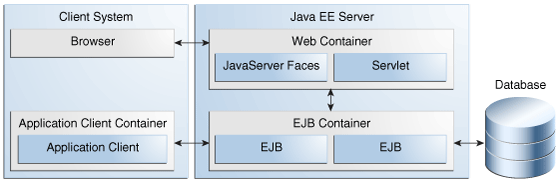
\includegraphics[width=\columnwidth]{containers.png}}
\end{frame}

\section{Composants}
\begin{frame}
	\frametitle{Composants}
	\begin{itemize}
		\item \emph{Composant} : une unité logicielle assemblée dans une application Java EE avec ses classes et fichiers liés et communiquant avec d’autres composants.
		\item Code Java compilé normalement
		\item Assemblé dans une application Java EE : peut utiliser les services ; doit se conformer aux spécifications
		\item Exécution gérée par le conteneur (pas de \texttt{main}, par exemple)
	\end{itemize}
\end{frame}

\begin{frame}
	\frametitle{Composant EJB}
	\begin{block}{EJB}
		\begin{itemize}
			\item \emph{Enterprise} Java Bean
			\item Composant \og{}business\fg{}, sur le serveur
			\item Service pouvant être appelé localement ou à distance
			\item Deux types : session bean, message-driven bean
		\end{itemize}
	\end{block}
	\begin{itemize}
		\item Le conteneur rend l’EJB accessible de l’extérieur
		\item Permet le Remote Method Invocation, sorte de RPC
		\item Le conteneur instancie, facilite la sérialisation, …
	\end{itemize}
\end{frame}

\begin{frame}
	\frametitle{Composant Web}
	\begin{itemize}
		\item Java Servlet {\tiny \href{http://www.oqlf.gouv.qc.ca/ressources/bibliotheque/dictionnaires/internet/fiches/8386532.html}{n. m.}}
		\item JavaServer Faces
	\end{itemize}
\end{frame}

\section{Couches}
\begin{frame}
	\frametitle{Couches (\og{}tier\fg{})}
	\begin{minipage}{\columnwidth*\real{0.6}}
		\href{https://docs.oracle.com/javaee/7/tutorial/overview003.htm}{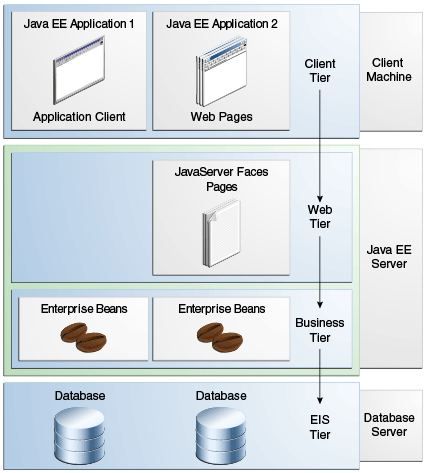
\includegraphics[width=\columnwidth]{tiers.png}}
	\end{minipage}%
	\begin{minipage}{\columnwidth*\real{0.4}}
		\begin{itemize}
			\item Ajout d’une couche multithread entre le client et le serveur classique
			\item Souvent : presentation, logic, data tier
			\item Couche web : peut être également appelé un client web (pourquoi ?).
		\end{itemize}
	\end{minipage}
\end{frame}

\begin{frame}
	\frametitle{Exemple d’application Java EE}
	\begin{itemize}
		\item Entreprise A : niveau de stock calculable d’après BDD
		\item Lib : requête pour obtenir le niveau de stock
		\item Web : servlet répondant à HTTP GET (client léger)
		\item Client Javascript (entreprise A)
		\item Client Java (entreprise B)
		\item Client Python (entreprise C)
	\end{itemize}		
\end{frame}

\section{Assemblage et déploiement}
\begin{frame}
	\frametitle{Modules}
	\begin{itemize}
		\item \emph{Module} Java EE : fichier archive compressé
		\item Ensemble de composants pour un même conteneur {\tiny (typiquement)}
		\item Éventuellement : un descripteur de déploiement (\texttt{.xml}) pour ce type de conteneur (standard Java EE ou par produit)
		\item Éventuellement :  des pages HTML statiques ; des classes utilité, …
		\item Les descripteurs surchargent les annotations
	\end{itemize}
\end{frame}

\begin{frame}
	\frametitle{Module Web}
	\begin{block}{Module Web}
		\begin{itemize}
			\item Fichier \texttt{.war}
			\item Fichiers \texttt{.class} servlets et autres dans WEB-INF/lib ou WEB-INF/classes
			\item Fichiers web statiques (.html, images, …) dans root
			\item \texttt{WEB-INF/web.xml} : descripteur pour conteneur Web
			\item \texttt{META-INF/glassfish-web.xml} : descripteur pour glassfish
			\item \texttt{META-INF/MANIFEST.MF}
		\end{itemize}
	\end{block}
%	\begin{block}{Module EJB}
%		\begin{itemize}
%			\item Fichier \texttt{.jar}
%			\item Fichiers \texttt{.class} EJB et autres
%			\item \texttt{META-INF/ejb-jar.xml} : descripteur pour conteneur EJB (attributs de transaction, sécurité, …)
%			\item \texttt{META-INF/glassfish-ejb-jar.xml} : descripteur pour glassfish
%			\item \texttt{META-INF/MANIFEST.MF}
%		\end{itemize}
%	\end{block}
%	\item Application client modules (class files and, optionally, an application client deployment descriptor) : \texttt{.jar}.
%	\item (Resource adapter modules : \texttt{.rar}.)
%    , which contain all Java interfaces, classes, native libraries, and, optionally, a resource adapter deployment descriptor. Together, these implement the Connector architecture (see Java EE Connector Architecture) for a particular EIS. Resource adapter modules are packaged as JAR files with an .rar (resource adapter archive) extension.
\end{frame}

\begin{frame}
	\frametitle{Assemblage et déploiement}
	\begin{itemize}
		\item Application Java EE composée d’un ou plusieurs modules
		\item On peut déployer un module seul (\texttt{.war}, \texttt{.jar})
		\item Ou assembler les modules dans un fichier Enterprise Archive (\texttt{.ear})
		\item EAR : plusieurs modules et év. descripteur d’application (\texttt{META-INF/application.xml}, \texttt{META-INF/glassfish-application.xml})
	\end{itemize}
	\begin{block}{Déploiement}
		\begin{itemize}
			\item Procédure dépend du serveur d’application Java EE
			\item Typiquement : déplacer l’archive (\texttt{.war}, \texttt{.ear}, \texttt{.jar}) dans un répertoire du serveur
			\item Accès depuis l’environnement de développement via plug-ins
		\end{itemize}
	\end{block}
\end{frame}

\section{Services}
\begin{frame}
	\frametitle{Services}
	Exemples :
	\begin{itemize}
		\item Managed beans
		\item CDI
		\item RestFul
		\item JSF
		\item Bean validation
		\item JAXB, JAX-WS, JNDI (aussi dans Java SE)
	\end{itemize}
\end{frame}

\section{GlassFish}
\begin{frame}
	\frametitle{GlassFish Server Tools}
	\begin{itemize}
		\item Démarrer, arrêter le serveur
		\item Déployer des paquets
		\item Application : console d’administration
		\item Base de données
	\end{itemize}
	\begin{block}{À vous}
		\begin{itemize}
			\item \og{}Installez\fg{} GlassFish (copie depuis \texttt{/usr/local/glassfish-4.1/glassfish})
			\item Démarrez votre serveur (cf. \texttt{bin/}, \url{http://localhost:8080}, \url{http://localhost:4848})
			\item Désactivez l’écoute extérieure
			\item Lisez les logs
		\end{itemize}
	\end{block}
\end{frame}

\appendix
\section{Licence}
\begin{frame}
	\frametitle{Licence}
	Cette présentation, et le code LaTeX associé, sont sous \href{https://opensource.org/licenses/MIT}{licence MIT}. Vous êtes libres de réutiliser des éléments de cette présentation, sous réserve de citer l’auteur.
	
	Le travail réutilisé est à attribuer à \href{http://www.lamsade.dauphine.fr/~ocailloux/}{Olivier Cailloux}, Université Paris-Dauphine.
\end{frame}
\section{Java}
\begin{frame}[fragile]
	\frametitle{Le terme Java}
	
	Terme \emph{Java} adopté en 1995 (“as an example of yet another name that would never work”) \source{(source: \href{https://www.javaworld.com/article/2077265/core-java/so-why-did-they-decide-to-call-it-java-.html}{Java World})}
	\hfill
	\vfill
	\begin{minipage}[b]{3cm}
		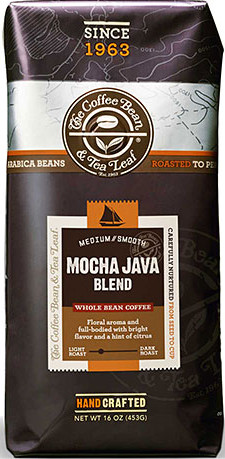
\includegraphics[height=5.5cm]{Java_beans.jpg}
	\end{minipage}%
	\begin{minipage}[b]{(\columnwidth - 3cm)}
		\centering{
\includegraphics[height=9mm]{java-icon.png}}
		\pause
		\href{https://en.wikipedia.org/wiki/Java}{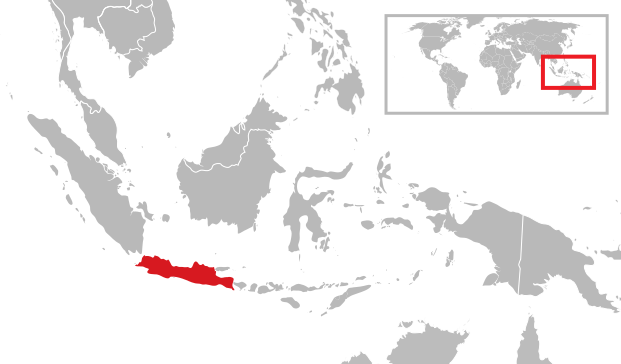
\includegraphics[width=\columnwidth]{Java_Locator.svg.png}}
%		\mbox{} \raggedleft \source{Gunawan Kartapranata - \href{https://en.wikipedia.org/wiki/Java}{wikipedia}}
	\end{minipage}
\end{frame}

\begin{frame}
	\frametitle{A jar full of Java beans, please}
	\begin{itemize}
		\item JAR File : introduits à la version 1.1. Une collection de fichiers \texttt{.class}.
		\item Java Bean (aussi version 1.1). (\href{http://www.oracle.com/technetwork/java/javase/documentation/spec-136004.html}{specs}) : un composant logiciel pour assemblage (par exemple, un bouton AWT, une feuille de calcul à placer dans un document).
	\end{itemize}
	\centering{
		\href{http://houseofjava.ca/}{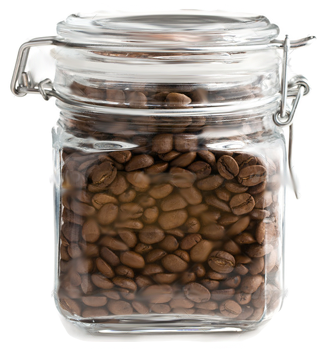
\includegraphics[height=3cm]{bean-jar.png}}
	}
	\begin{block}{Fun fact}
		Voyons le nombre magique des fichiers \texttt{.class}…
	\end{block}
\end{frame}

\section{Session HTTP}
\begin{frame}
	\frametitle{Servlet et session HTTP}
	\begin{itemize}
		\item Un servlet s’exécute dans un contexte
		\item Entre autres, une session HTTP
		\item Objet \href{https://docs.oracle.com/javaee/7/api/javax/servlet/http/HttpSession.html}{\texttt{HttpSession}} rendu disponible par conteneur ({\tiny injection ou } accès via paramètres servlet)
		\item Le serveur tente de tracker la session via un cookie {\tiny par exemple}
		\item Le serveur fait expirer le cookie après un temps configurable
		\item Un bon site fonctionne même sans cookies !
		\item Classe implémente \href{https://docs.oracle.com/javaee/7/api/javax/servlet/http/HttpSessionListener.html}{\texttt{HttpSessionListener}} pour recevoir notifications \texttt{sessionCreated}, \texttt{sessionDestroyed}.  L’annoter \href{https://docs.oracle.com/javaee/7/api/javax/servlet/annotation/WebListener.html}{\texttt{@WebListener}}. (Pattern ? \pause Observateur !)
	\end{itemize}
\end{frame}

%\subsection{Détails}
%\begin{frame}
%	\frametitle{Servlet (trop de détails)}
%	\begin{itemize}
%		\item Le servlet peut accéder à des objets via getAttribute et setAttribute d’une classe représentant un scope : sur ServletContext, HttpSession, ServletRequest. Il faut se protéger contre les accès concurrents !
%		\item HTTP request URL : http ://host:portrequestpath?querystring, with
%		\item requestpath=contextpathservletpathpathinfo, with 
%		\item contextpath=/contextroot (of the servlet’s web app) or "", 
%		\item servletpath=The path section that corresponds to the component alias that activated this request. This path starts with a forward slash (/) (or is empty), pathinfo = the rest.
%	\end{itemize}
%\end{frame}

\end{document}

\begin{frame}
	\frametitle{}
	\begin{itemize}
		\item 
	\end{itemize}
	\begin{block}{}
		
	\end{block}
\end{frame}

\section{Bibliographie}
\begin{frame}[allowframebreaks]
	\frametitle{Bibliographie}
	\def\newblock{\hskip .11em plus .33em minus .07em}
% 	\bibliography{zotero}
\end{frame}

\section{Autres}
\begin{frame}
	\frametitle{}
	\begin{itemize}
		\item 
	\end{itemize}
	\begin{block}{}
		
	\end{block}
\end{frame}
\end{document}
